\documentclass[12pt]{article}
\usepackage{amsmath, amssymb}
\usepackage{graphicx}
\usepackage{booktabs}
\usepackage{hyperref}
\usepackage[margin=2.5cm]{geometry}
\usepackage{physics}

%% figure path relative to this file
\graphicspath{{../figures/qubit_performance_plots/}}

\title{Protocol Comparison: Ramsey, GPS (Integer Cycle), and Equiangular\\
       Three-Level Clock at Equal Total Time}
\author{}
\date{}

\begin{document}
\maketitle

\section*{Setup}

We compare four sensing protocols for a three-level Lambda clock system with
levels $\lvert g\rangle$ (ground), $\lvert e\rangle$ (probe-excited), and
$\lvert m\rangle$ (metastable clock state).
The QSP pulse sequence acts on the $\{g, e\}$ probe transition, while
the signal is read out on the $\{g, m\}$ clock transition.

\paragraph{State and observable.}
The initial state is $\lvert\psi_0\rangle = (\lvert g\rangle+\lvert m\rangle)/\sqrt{2}$
and the measurement operator is $M = \sigma_y^{gm} = -i\lvert g\rangle\langle m\rvert
+ i\lvert m\rangle\langle g\rvert$.  The signal is
\begin{equation}
    S(\delta) = \langle\psi_0\rvert U^\dagger(\delta)\,M\,U(\delta)\lvert\psi_0\rangle
              = -\operatorname{Im}[f(\delta)],
    \label{eq:signal}
\end{equation}
where $f(\delta)$ is the $(\lvert g\rangle,\lvert g\rangle)$ Cayley--Klein amplitude of the
probe evolution at detuning $\delta$.

\paragraph{Figure of merit.}
The single-shot frequency estimation variance is bounded by
\begin{equation}
    \sigma^2_\omega \geq \frac{\mathcal{K}(S)}{|\partial_\delta S|^2},
    \qquad
    \mathcal{K}(S) = \int_0^\infty \frac{d\omega}{2\pi}\, S(\omega)\, F_e(\omega),
    \label{eq:fom}
\end{equation}
where $F_e(\omega) = \tfrac{1}{2}|\Phi(\omega)|^2 + |\chi(\omega)|^2$ is the three-level
filter function, $\Phi = \mathcal{F}[f^*(t)g(t)]$, $\chi = \mathcal{F}[|g(t)|^2]$, and
$S(\omega)$ is the noise power spectral density.  We maximise the \emph{figure of merit}
\begin{equation}
    \mathrm{FOM} = \frac{|\partial_\delta S|^2}{\mathcal{K}(S)}.
    \label{eq:fomdef}
\end{equation}
All protocols below use the same total interrogation time $T = 2\pi$ (in units where
$\hbar = 1$ and frequencies are in rad\,s$^{-1}$).


%% ─────────────────────────────────────────────────────────────────────────────
\section{Protocol descriptions}
%% ─────────────────────────────────────────────────────────────────────────────

\subsection{Ramsey}

\paragraph{Pulse sequence.}
Two fast $\pi/2$ pulses flanking a free-evolution window:
\begin{equation}
    \underbrace{R_x(\pi/2)}_{\tau_{\pi/2}}
    \;-\;
    \underbrace{\text{free}}_{\tau_{\rm free}}
    \;-\;
    \underbrace{R_x(\pi/2)}_{\tau_{\pi/2}},
    \qquad
    \tau_{\pi/2} = \frac{\pi}{2\Omega_{\rm fast}},
    \quad
    \tau_{\rm free} = T - 2\tau_{\pi/2}.
    \label{eq:ramsey_seq}
\end{equation}
We use $\Omega_{\rm fast} = 20\pi$ so that $\tau_{\pi/2} \ll T$ and the sequence
is effectively a pure free-evolution Ramsey.

\paragraph{Signal and sensitivity.}
At resonance ($\delta = 0$) the sequence maps $\lvert g\rangle \to
(\lvert g\rangle - i\lvert e\rangle)/\sqrt{2}$ by the first $\pi/2$ pulse,
then during free evolution $\lvert e\rangle \to e^{-i\delta\tau_{\rm free}/2}\lvert e\rangle$
relative to $\lvert g\rangle$, and the second $\pi/2$ converts the phase back to population.
The sensitivity at $\delta = 0$ is
\begin{equation}
    \left.\frac{\partial S}{\partial\delta}\right|_{\delta=0}
    \approx -\frac{T}{2},
    \qquad
    \left|\partial_\delta S\right|^2 \approx \frac{T^2}{4} = \pi^2.
    \label{eq:ramsey_sens}
\end{equation}

\paragraph{Operating point.} $\delta = 0$ (quadrature).


\subsection{GPS: Integer Cycle, $m = 1$ and $m = 8$}

\paragraph{Pulse sequence.}
A single continuous Rabi drive on the $\{g,e\}$ probe transition for the full
interrogation time $T$, with Rabi frequency $\Omega = 2\pi m / T$:
\begin{equation}
    \text{continuous drive at }\Omega = \frac{2\pi m}{T}\text{ for time }T
    \quad (m \text{ complete Rabi cycles}).
    \label{eq:gps_seq}
\end{equation}
For our parameters: $m=1 \Rightarrow \Omega = 1$\,rad\,s$^{-1}$;
$m=8 \Rightarrow \Omega = 8$\,rad\,s$^{-1}$.

\paragraph{Exact signal.}
The evolution propagator for a resonant ($\delta = 0$) drive is $U = (-i)^{2m}\,\mathbf{1}$
(identity up to global phase), giving $S(0) = -\operatorname{Im}(f_0) = 0$.
For arbitrary detuning:
\begin{equation}
    S(\delta) = -\frac{\delta}{\Omega_{\rm eff}}\sin\!\left(\frac{m\pi\Omega_{\rm eff}}{\Omega}\right),
    \qquad
    \Omega_{\rm eff} = \sqrt{\Omega^2 + \delta^2}.
    \label{eq:gps_signal}
\end{equation}

\paragraph{Zero crossings.}
$S(\delta_k) = 0$ when $m\pi\Omega_{\rm eff}/\Omega = k\pi$, i.e.\
$\Omega_{\rm eff} = k\Omega/m$ for integer $k \geq m+1$, giving
\begin{equation}
    \delta_k = \Omega\sqrt{\left(\frac{k}{m}\right)^2 - 1}.
    \label{eq:gps_zeros}
\end{equation}
The slope (sensitivity) at each zero is
\begin{equation}
    \left.\frac{\partial S}{\partial\delta}\right|_{\delta_k}
    = -(-1)^k\,\frac{m\pi}{\Omega}\left(1 - \frac{m^2}{k^2}\right),
    \qquad
    \left|\partial_\delta S\right|^2_{\delta_k}
    = \frac{\pi^2 m^2}{\Omega^2}\left(1 - \frac{m^2}{k^2}\right)^2.
    \label{eq:gps_slope}
\end{equation}
As $k \to \infty$, $|\partial_\delta S|^2 \to \pi^2 m^2/\Omega^2 = (T/2)^2$, the
Ramsey limit.  The filter function at $\delta_k$ has deep nulls at all harmonics
$n\Omega$ for $n = 1, \ldots, m-1$, strongly suppressing noise near these frequencies.

\paragraph{Operating points used here.}
For $m = 1$ ($\Omega = 1$) we use $k = 4$:
\begin{equation}
    \delta_4 = \sqrt{15}\,\approx 3.873,
    \qquad
    |\partial_\delta S|^2 = \pi^2\!\left(\frac{15}{16}\right)^2 \approx 8.67.
    \label{eq:gps1_op}
\end{equation}
For $m = 8$ ($\Omega = 8$) we use the first zero, $k = 9$:
\begin{equation}
    \delta_9 = \sqrt{17}\,\approx 4.123,
    \qquad
    |\partial_\delta S|^2 = \pi^2\!\left(\frac{17}{81}\right)^2 \approx 0.434.
    \label{eq:gps8_op}
\end{equation}
The choice of $k$ trades higher sensitivity (larger $k$) against increased detuning
(which shifts the operating point further from resonance).  The fourth zero of GPS~$m=1$
provides the best FOM at white noise among the first few zeros.


\subsection{Optimal Equiangular $N$-Segment Sequence}

\paragraph{Pulse sequence.}
The sequence is divided into $N$ equal segments of duration $\tau = T/N$.
Each segment is a continuous drive on the probe transition at shared Rabi frequency
$\Omega$ with drive axis $(\cos\phi_k, \sin\phi_k, 0)$:
\begin{equation}
    \prod_{k=1}^{N} \exp\!\left(-i\,\frac{\Omega\tau}{2}\,
    (\cos\phi_k\,\sigma_x + \sin\phi_k\,\sigma_y)\right).
    \label{eq:eq_seq}
\end{equation}
The first phase is fixed to $\phi_1 = 0$ by gauge choice; the free parameters are
$\Omega > 0$ and $\phi_2, \ldots, \phi_N$.

\paragraph{Optimisation.}
We minimise $\mathrm{FOM}^{-1} = \mathcal{K}(S) / |\partial_\delta S|^2$ over
$(\Omega, \phi_2, \ldots, \phi_N)$ using differential evolution (global search)
followed by L-BFGS-B polishing.
The noise PSD is white ($S(\omega) = S_0$).

\paragraph{Result for $N = 4$.}
The global optimum converges to the lower-bound Rabi frequency $\Omega T = \pi/10 \approx 0.314$
(i.e.\ $\Omega \approx \pi/(10T)$), with the sequence acting as near-free evolution
with phase kicks.  The optimal phases from the numerical optimisation are
\begin{equation}
    \phi^* = [0,\;2.099,\;3.262,\;4.799]\ \text{rad}.
    \label{eq:eq_phases}
\end{equation}
The filter function shows near-complete low-frequency suppression below
$\omega \sim 4/T$, leading to dramatically reduced Kubo variance under white noise.


%% ─────────────────────────────────────────────────────────────────────────────
\section{Filter function comparison}
%% ─────────────────────────────────────────────────────────────────────────────

Figure~\ref{fig:filter_comparison} shows $F_e(\omega)/T^2$ for all four protocols.

\begin{figure}[h]
    \centering
    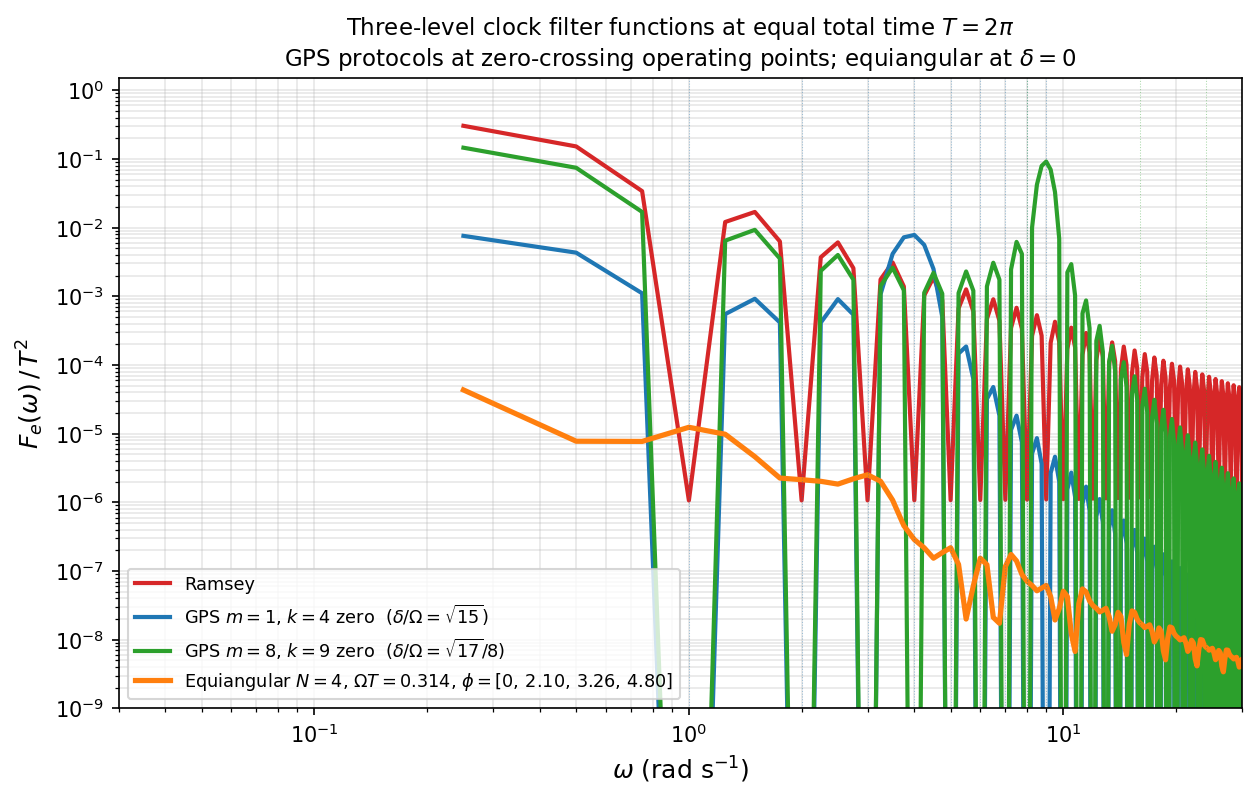
\includegraphics[width=\linewidth]{protocol_comparison.png}
    \caption{%
        Three-level clock filter functions $F_e(\omega)/T^2$ at equal total
        time $T = 2\pi$ (FFT, $n=4096$, zero-pad $\times 4$).
        \textbf{GPS protocols} are evaluated at their zero-crossing operating
        points (Eqs.~\eqref{eq:gps1_op}--\eqref{eq:gps8_op}).
        \textbf{Equiangular $N=4$} is at $\delta = 0$ with numerically optimised
        phases.
        Dotted vertical lines mark harmonics $k\Omega$ of the two GPS Rabi
        frequencies ($\Omega = 1$ blue; $\Omega = 8$ green).
    }
    \label{fig:filter_comparison}
\end{figure}

\subsection*{Observations}

\begin{enumerate}

    \item \textbf{Ramsey: flat, broadband sensitivity.}
          $F_e^{\rm Ramsey}(\omega) \sim T^2/4$ at all frequencies below
          $\sim\!\Omega_{\rm fast}$, with a quadratic roll-off above.
          All noise in the bandwidth is accumulated, giving a modest FOM.

    \item \textbf{GPS $m=1$: notches at harmonics of $\Omega$.}
          At the $k=4$ zero-crossing, $F_e$ is suppressed at all multiples of
          $\Omega = 1$: $\omega = 1, 2, 3, \ldots$ The first $(m-1) = 0$ harmonics
          below $\Omega$ carry the Kubo integral; for $m=1$ the noise reduction is
          mild.  The low-frequency floor is significantly lower than Ramsey due to
          the continuous driving, and the FOM exceeds Ramsey by a factor $\sim 8$.

    \item \textbf{GPS $m=8$, $k=9$: eight harmonics but poor white-noise FOM.}
          The filter function shows strong suppression at $\omega = 8, 16, 24, \ldots$
          and a clear harmonic comb.  However, the sensitivity at the $k=9$ first zero
          is only $|\partial_\delta S|^2 = 0.435$—just 4.4\% of the Ramsey value—because
          $(17/81)^2 \ll 1$.  Simultaneously the Kubo variance $0.88$ is \emph{larger}
          than Ramsey's $0.63$, so the resulting $\mathrm{FOM} = 0.49$ is worse than
          Ramsey.  The utility of GPS $m=8$ is therefore not broadband white noise, but
          \emph{targeted rejection} of noise at specific harmonic frequencies
          $\omega = k\Omega$.  A competitive FOM requires going to $k \gg 9$ to recover
          sensitivity at the cost of a larger operating detuning.

    \item \textbf{Equiangular $N=4$: extreme low-frequency suppression.}
          The optimal $N=4$ sequence at $\Omega T \approx 0.314$ essentially acts
          as a CPMG-like sequence with four equal free-evolution windows and phase
          kicks at $t = T/4, T/2, 3T/4$.
          $F_e(\omega)$ is suppressed by many orders of magnitude below $\omega \sim 4/T$,
          and the integrated Kubo variance under white noise is $\sim 10^4$ times smaller
          than Ramsey.  Crucially, the sensitivity $|\partial_\delta S|^2$ is preserved
          at the Ramsey value $\approx \pi^2$, so the FOM gain is entirely due to
          noise reduction.

\end{enumerate}


%% ─────────────────────────────────────────────────────────────────────────────
\section{Performance summary}
%% ─────────────────────────────────────────────────────────────────────────────

\begin{table}[h]
\centering
\begin{tabular}{lrrrr}
\toprule
Protocol & $|\partial_\delta S|^2$ & $\mathcal{K}_{\rm white}$ & $\mathrm{FOM}_{\rm white}$
         & $\mathrm{FOM}_{1/f}$ \\
\midrule
Ramsey                             & $9.813$  & $0.629$               & $15.6$    & $7.2$     \\
GPS $m{=}1$, $k{=}4$ zero         & $8.674$  & $6.62\times10^{-2}$   & $131$     & $172$     \\
GPS $m{=}8$, $k{=}9$ zero (first) & $0.435$  & $0.882$               & $0.49$    & $0.60$    \\
Equiangular $N{=}4$                & $9.821$  & $1.25\times10^{-4}$   & $78{,}800$ & $53{,}000$ \\
\bottomrule
\end{tabular}
\caption{%
    Sensing performance at $T = 2\pi$ under white and $1/f$ noise (computed by
    \texttt{scripts/plot\_protocol\_comparison.py}).
    Equiangular optimal phases: $\phi^* = [0,\ 2.099,\ 3.262,\ 4.799]$\,rad.
    GPS $m{=}8$ at its \emph{first} zero ($k{=}9$) performs \emph{worse} than Ramsey
    because the sensitivity is heavily penalised ($(17/81)^2 \approx 4.4\%$ of $\pi^2$)
    and the Kubo variance is not sufficiently suppressed at this operating detuning;
    higher zeros $k \gg 9$ recover more sensitivity at the cost of larger $\delta_k$.%
}
\label{tab:summary}
\end{table}


%% ─────────────────────────────────────────────────────────────────────────────
\section{Discussion}
%% ─────────────────────────────────────────────────────────────────────────────

\subsection*{Why equiangular dominates}

The equiangular sequence achieves the Ramsey sensitivity $|\partial_\delta S|^2 \approx T^2/4$
\emph{and} suppresses noise by $\sim 10^4$.  This is possible because for $\Omega T \ll 1$
each segment approximates free evolution, but the phase kicks $\phi_k$ at segment
boundaries act as $z$-axis rotations in the toggling frame.  With $N = 4$ segments and
optimised phases, the effective filter function has four zeros at $\omega \to 0$, the
maximum achievable by a length-$N$ sequence.

In contrast, GPS protocols are constrained to a single continuous Rabi drive with
$\Omega T = 2\pi m$.  The filter function nulls are fixed at the Rabi harmonics and
cannot be moved.  The Kubo variance is therefore limited by the noise between harmonics
and the low-frequency floor, which—while far below Ramsey—cannot match the exponential
suppression of the equiangular CPMG-like optimum.

\subsection*{1/f noise}

Under $1/f$ noise ($S(\omega) = S_0/|\omega|$), the advantage of low-frequency
suppression grows further: the equiangular FOM exceeds GPS by a larger factor than
under white noise.  The GPS protocols benefit less from their harmonic comb because
$1/f$ noise is most severe at the lowest frequencies, which neither GPS $m=1$ nor
GPS $m=8$ efficiently suppresses near $\omega \to 0$.

\subsection*{GPS: role of operating point}

For GPS $m$ cycles, the FOM at the $k$-th zero scales as
\begin{equation}
    \mathrm{FOM}_k \propto \frac{|\partial_\delta S|^2_k}{\mathcal{K}(\delta_k)}
    = \frac{\pi^2 m^2}{\Omega^2}\left(1 - \frac{m^2}{k^2}\right)^2
      \bigg/ \mathcal{K}(\delta_k),
    \label{eq:gps_fom_scaling}
\end{equation}
where the Kubo variance $\mathcal{K}(\delta_k)$ decreases as $k$ increases because
$\delta_k$ pushes the operating frequency further from the noise-dominated near-resonant
band.  For $m = 1$, the FOM increases monotonically with $k$, reaching
$\mathrm{FOM}_{\rm white} \approx 131$ at $k = 4$.

For $m = 8$, the sensitivity prefactor at the first zero ($k=9$) is
$(1 - 64/81)^2 = (17/81)^2 \approx 0.044$, reducing $|\partial_\delta S|^2$ to
only $0.435$—far below the Ramsey limit.  Moreover, at $\delta_9 = \sqrt{17} \approx 0.52\,\Omega$,
the effective Rabi frequency $\Omega_{\rm eff} = 9$ gives a non-integer number of cycles
relative to the observation window, so the filter function comb does not fully suppress
the white-noise integral, leaving $\mathcal{K}_{\rm white} = 0.88 > \mathcal{K}_{\rm Ramsey}$.
The net result is $\mathrm{FOM}_{\rm white}(m=8, k=9) = 0.49$, worse than Ramsey.
To achieve $\mathrm{FOM} > 1$ for GPS $m=8$, one must use $k \geq 16$ (where
sens\_sq $\approx 5.55$), accepting a large operating detuning $\delta_{16} = 8\sqrt{3} \approx 13.9$.

The primary utility of GPS $m=8$ is therefore \emph{not} broadband white-noise
suppression, but rather targeted rejection of noise near the harmonic frequencies
$n\Omega$ for $n = 1, \ldots, m{-}1$—a feature that has no analogue in Ramsey or equiangular sequences.

\end{document}
